\documentclass[12pt]{article}
\newenvironment{problem}[2][Problem]{\begin{trivlist}
\item[\hskip \labelsep {\bfseries #1}\hskip \labelsep {\bfseries #2.}]}{\end{trivlist}}
\usepackage{amssymb}
\usepackage{amsmath}
\usepackage{fancyhdr}

\usepackage{enumitem}
\usepackage{graphicx}
\usepackage{hyperref}
\usepackage{color}

\usepackage{etoolbox,refcount}
\usepackage{multicol}

\newcounter{countitems}
\newcounter{nextitemizecount}
\newcommand{\setupcountitems}{%
  \stepcounter{nextitemizecount}%
  \setcounter{countitems}{0}%
  \preto\item{\stepcounter{countitems}}%
}
\makeatletter
\newcommand{\computecountitems}{%
  \edef\@currentlabel{\number\c@countitems}%
  \label{countitems@\number\numexpr\value{nextitemizecount}-1\relax}%
}
\newcommand{\nextitemizecount}{%
  \getrefnumber{countitems@\number\c@nextitemizecount}%
}
\newcommand{\previtemizecount}{%
  \getrefnumber{countitems@\number\numexpr\value{nextitemizecount}-1\relax}%
}
\makeatother    
\newenvironment{AutoMultiColItemize}{%
\ifnumcomp{\nextitemizecount}{>}{3}{\begin{multicols}{2}}{}%
\setupcountitems\begin{itemize}}%
{\end{itemize}%
\unskip\computecountitems\ifnumcomp{\previtemizecount}{>}{3}{\end{multicols}}{}}


% \begin{itemize}
%     \item Here are two columns
%   \begin{AutoMultiColItemize}
%   \item Item 1
%   \item Item 2
%   \item Item 3
%   \item Item 4
%   \item Item 5
%   \item Item 6
%   \end{AutoMultiColItemize}
%   \item AutoMultiColItemize can be nested in an itemize
%   \item Or it does not have to be.
%   \item Normal itemize, like this one, are still single column.
% \end{itemize}
% Here is one column
% \begin{AutoMultiColItemize}
% \item Item 1
% \item Item 2
% \item Item 3
% \end{AutoMultiColItemize}


\begin{document}

\pagestyle{fancy}
\fancyhf{}
\lhead{GEOL 362A -- PS 2}
\rhead{Due: 8 Oct 2021}

% \title{Problem Set 1}
% % \author{GEOL 362A, Middlebury College}
% % \date{Due: 24 Sept 2021}
% \maketitle

\noindent The goal of this problem set is to practice applying conservation laws and force budget techniques to find useful information about a glacier.  Make sure to describe and motivate any necessary physical assumptions in your solution writeup.

%%%%%
\begin{problem}{1}
[7 pts] In the previous problem set, you produced a conservation equation for an idealized glacier in equilibrium with its climate:
\begin{equation}\label{eq:masscon}
    \int_0^L \alpha (h-E) \;\text{d}x =0,
\end{equation}
where $L$ is the glacier length, $h$ its surface elevation, $E$ its equilibrium line altitude, and $x$ the along-flow direction.  The surface elevation $h(x) = b_0 - sx + H$, where $b$ is the bed elevation at $x=0$, $s$ is a constant linear slope, and $H$ is the ice thickness.
\renewcommand{\labelenumi}{(\alph{enumi})}
\begin{enumerate}[itemsep=2pt]
    \item Using Equation \ref{eq:masscon} and the approach we demonstrated in class, show the steps to find an approximation of glacier length change resulting from equilibrium line elevation change, $\frac{\partial L}{\partial E}$.  You can assume perfectly plastic deformation, as we did in class, so the driving stress $\tau_{dx}$ must be balanced by a constant yield stress $\tau_0$.

    \item Now, consider the Alpine glacier Vernagtferner, shown in profile in Figure \ref{fig:vernagtferner}.  Estimate the length change that would result from a change in equilibrium line altitude for this glacier.
    
    \item Download two datasets from the internet:
        \begin{itemize}
            \item Davaze \& Rabatel dataset ``Annual glacier equilibrium-line altitude (ELA) for 239 glaciers located in the European Alps quantified from optical remote sensing data from 2000 to 2016'' [\textcolor{blue}{\href{https://www.theia-land.fr/en/product/annual-glacier-equilibrium-line-altitude/}{link}}, also on Canvas]. Extract the ELA history for Vernagtferner (you may do this manually or by coding; let me know which you do);
            \item Vernagtferner frontal variation, ``FoG\_FVobs\_489.csv'' from the World Glacier Monitoring Service [\textcolor{blue}{\href{https://wgms.ch/products_ref_glaciers/vernagtferner-alps/}{link}}].
        \end{itemize}
    Compute the true glacier length change observed per change in equilibrium line altitude during the 2000-2016 period.

    \item Is the equation we derived in class a suitable approximation for Vernagtferner?  Why or why not?
\end{enumerate}

\begin{figure}
    \centering
    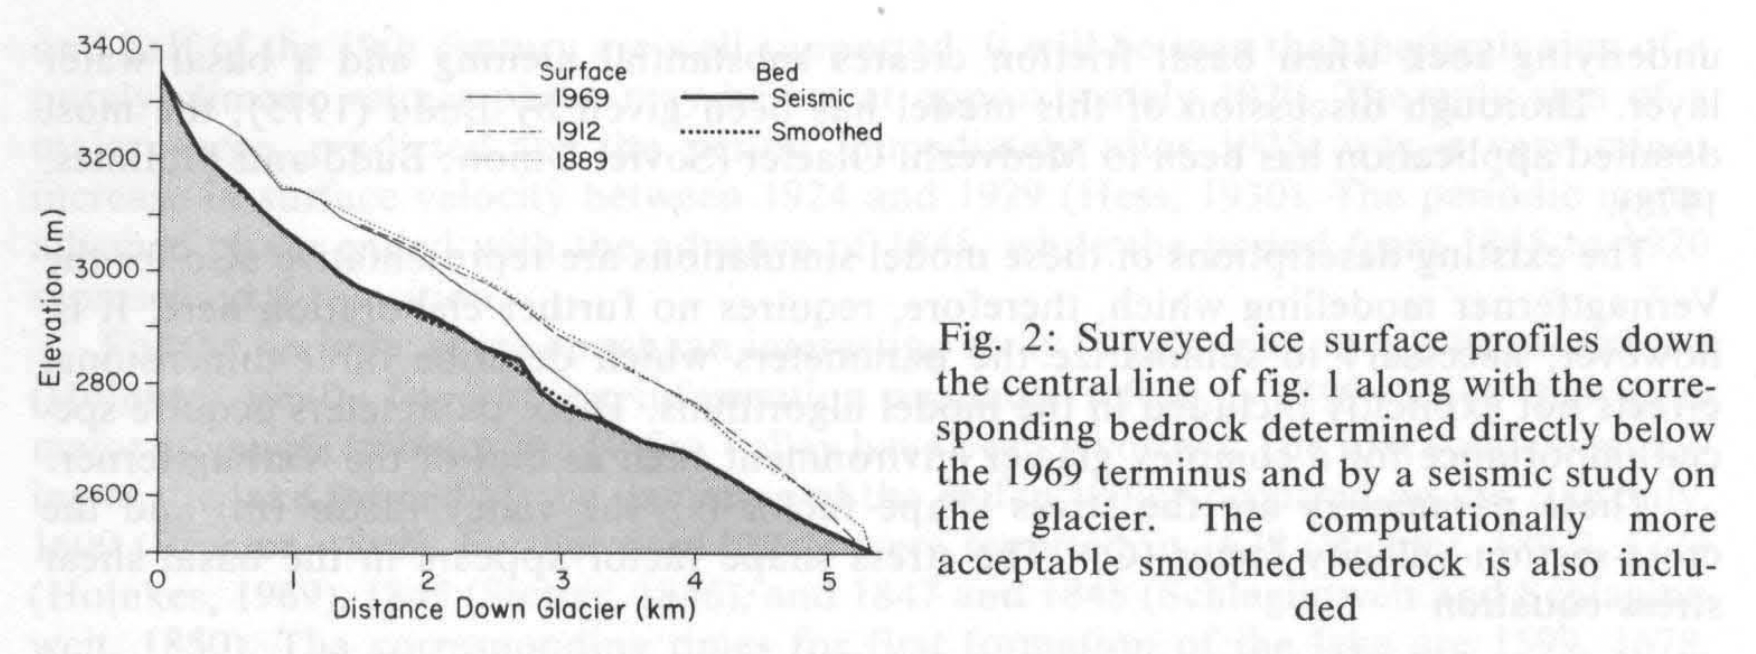
\includegraphics[width=0.9\linewidth]{figs/Screen Shot 2021-10-01 at 2.13.57 PM.png}
    \caption{Observed profile of Vernagtferner surface and bed elevation.\footnotemark}
    \label{fig:vernagtferner}
\end{figure}
\footnotetext{P.D. Kruss and I.N. Smith (1982) ``Numerical modelling of the Vernagtferner and its fluctuations'', \textit{Zeitschr. Gletscherkunde \& Glazialgeologie 18}(1):93-106.}
\end{problem}


\begin{problem}{2}
[5 pts] Consider a laterally symmetric ice stream with a thickness of $H=1100$ m thick, half-width of $W=15$ km, a density of $\rho = 910 \:\text{kg}^3\text{m}^{-3}$, and an along-flow slope of $\frac{\partial h}{\partial x} = 1.3 \times 10^{-3}$. The shear stress has been measured at one glacier margin to be $1.7 \times 10^5$ Pa and is assumed to be constant with ice thickness. Assume that the ice stream is rectangular in shape and assign a coordinate system with $x$ pointing along flow. 
\renewcommand{\labelenumi}{(\alph{enumi})}
\begin{enumerate}[itemsep=2pt]
    \item Compute the average along-flow gravitational driving stress of this ice stream.
    \item Compute the width-averaged lateral drag from the margins (van der Veen Section 4.4).
    \item What fraction of the driving stress is balanced by lateral drag in this case?  What contribution to the force balance do you expect from basal drag?
\end{enumerate}
\end{problem}


%%%%%
\begin{problem}{3}
[3 pts] In general, solving systems of PDEs is hard.  We therefore make use of simplifying approximations wherever possible.  For each of the following, outline the assumptions that must be satisfied and provide an example of a glaciological setting where the approximation \textbf{is not} suitable.
\renewcommand{\labelenumi}{(\alph{enumi})}
\begin{enumerate}[itemsep=2pt]
    \item Shallow Ice Approximation controlled by basal drag
    \item Shallow Ice Approximation controlled by lateral drag
    \item Shallow Shelf Approximation
\end{enumerate}

\end{problem}


\end{document}